\documentclass[fleqn,a4paper,12pt]{article}
\usepackage{standalone}		% Zum Einlesen aus anderen .tex-Files
\usepackage{geometry}		% Zur Bearbeitung des Layouts (Ränder,...)
\geometry{left=30mm, right=40mm, bottom=30mm}
\usepackage[german]{babel}
\usepackage[utf8]{inputenc}
\usepackage{amsmath}		% Mathematische Symbole
\usepackage{amssymb}     	% Nochmehr mathematische Symbole
\usepackage{dsfont}      	% Schriftsatz fuer Zahlenmengensymbole
%\usepackage{verbatim}   	% erweiterte Verbatim-Umgebung
\usepackage{alltt}       	% Quasi-Verbatim-Umgebung
\usepackage{fancyhdr}    	% Eigene Kopfzeilen
\usepackage{graphicx}    	% Zum Einbinden von Grafiken
% Einbinden einer eps-Grafik geht so: includegraphics{path}
\usepackage{wrapfig}
\usepackage{lscape}
\usepackage{rotating}
\usepackage{epstopdf}

% Seitenraender
\addtolength{\voffset}{-2cm}
\addtolength{\textheight}{0cm}
\addtolength{\hoffset}{0cm}
\addtolength{\textwidth}{2cm}
\addtolength{\headheight}{2cm} % fuer jeden Strichkode einen Zentimeter

% Skalierung der Grafiken
\setlength{\unitlength}{1cm}

\pagestyle{fancy}            % Eigene Kopfzeilen verwenden
\frenchspacing               % Kein Extrafreiraum nach Satzzeichen
\setlength{\parindent}{0pt}  % Neue Absaetze nicht einruecken
%\sloppy                     % Schlampige Absatzformatierung
\fussy                       % Penible Absatzformatierung
\linespread{1.5}             % Zeilenabstand

% Font fuer Code 39
\font\xlix=wlc39 scaled 1200
\newcommand\barcode[1]{{\xlix@#1@}}

% Name, Matrikelnummer, Barcode
\newcommand\student[2]{
\mbox{\scriptsize
	\begin{tabular}{@{}l@{}r@{}}
		\multicolumn{2}{@{}r@{}}{\barcode{#2}}\\
		#1&#2\\
	\end{tabular}}}

%andere Definitionen
\newcommand{\R}{{\mathbb R}}
\newcommand{\N}{{\mathbb N}}
\newcommand{\Z}{{\mathbb Z}}
\newcommand{\Q}{{\mathbb Q}}
\newcommand{\C}{{\mathbb C}}
\newcommand{\F}{\mathcal{F}}
\newcommand{\less}{\setminus}
\newcommand{\inv}{{}^{-1}}
\newcommand{\Land}{\bigwedge}
\newcommand{\Lor}{\bigvee}

% Kopfzeile
\lhead{
	\small
	\textsc{Grundlagen der Signalverarbeitung \\
		WS 2017/2018 \\
		Übung (\today)}
	\vfill}
\rhead{
	\begin{tabular}[b]{@{}rr@{}}
		\student{Philipp Badenhoop}{572693} &
		\student{Steven Lange}{568733} \\
		\student{Pascal Jochmann}{575056} &
		\student{Kevin Trogant}{572451}
	\end{tabular}}

\begin{document}
	\documentclass[fleqn,a4paper,12pt]{article}

%used Packages
\usepackage{standalone}		% Zum Einlesen aus anderen .tex-Files
\usepackage{geometry}		% Zur Bearbeitung des Layouts (Ränder,...)
\usepackage[german]{babel}
\usepackage[utf8]{inputenc}
\usepackage{amsmath}		% Mathematische Symbole
\usepackage{amssymb}     	% Nochmehr mathematische Symbole
\usepackage{dsfont}      	% Schriftsatz fuer Zahlenmengensymbole
%\usepackage{verbatim}   	% erweiterte Verbatim-Umgebung
\usepackage{alltt}       	% Quasi-Verbatim-Umgebung
\usepackage{fancyhdr}    	% Eigene Kopfzeilen
\usepackage{graphicx}    	% Zum Einbinden von Grafiken
							% Einbinden einer eps-Grafik geht so: includegraphics{path}
\usepackage{wrapfig}
\usepackage{lscape}
\usepackage{rotating}
\usepackage{epstopdf}

% Skalierung der Grafiken
\setlength{\unitlength}{1cm}

\frenchspacing               % Kein Extrafreiraum nach Satzzeichen
\setlength{\parindent}{0pt}  % Neue Absaetze nicht einruecken
%\sloppy                     % Schlampige Absatzformatierung
\fussy                       % Penible Absatzformatierung
\linespread{1.5}             % Zeilenabstand


% Seitenraender
\geometry{left=30mm, right=40mm, bottom=30mm}
				% Doc-class, Packageimports, fancy stuff
%%Seitenränder formatieren
\addtolength{\voffset}{-2cm}
\addtolength{\textheight}{0cm}
\addtolength{\hoffset}{0cm}
\addtolength{\textwidth}{2cm}
\addtolength{\headheight}{2cm} % fuer jeden Strichkode einen Zentimeter

% Font fuer Code 39
\font\xlix=wlc39 scaled 1200
\newcommand\barcode[1]{{\xlix@#1@}}

% Name, Matrikelnummer, Barcode
\newcommand\student[2]{
	\mbox{\scriptsize
		\begin{tabular}{@{}l@{}r@{}}
			\multicolumn{2}{@{}r@{}}{\barcode{#2}}\\
			#1&#2\\
		\end{tabular}}}

% Kopfzeile
\pagestyle{fancy}            % Eigene Kopfzeilen verwenden
\lhead{
	\small
	\textsc{Grundlagen der Signalverarbeitung \\
		WS 2017/2018 \\
		\"Ubung (\today)}
	\vfill}
\rhead{
	\begin{tabular}[b]{@{}rr@{}}
		\student{Philipp Badenhoop}{572693} &
		\student{Steven Lange}{568733} \\
		\student{Pascal Jochmann}{575056} &
		\student{Kevin Trogant}{572451}
\end{tabular}}			% Definition der Kopfzeile
%andere Definitionen
\providecommand{\R}{{\mathbb R}}
\providecommand{\N}{{\mathbb N}}
\providecommand{\Z}{{\mathbb Z}}
\providecommand{\Q}{{\mathbb Q}}
\providecommand{\C}{{\mathbb C}}
\providecommand{\F}{\mathcal{F}}
\providecommand{\less}{\setminus}
\providecommand{\inv}{{}^{-1}}
\providecommand{\Land}{\bigwedge}
\providecommand{\Lor}{\bigvee}			% Liste der zusätzlichen Commands und redefines

\begin{document}    
    \section*{Übungsaufgabe 13}
    \begin{tabular}{ | l | l | }
        \hline
        Signal & schwach stationär \\ \hline
        1 & ja \\ \hline
        2 & nein \\ \hline
        3 & nein \\ \hline
    \end{tabular}
    \newline \newline
    Begründung: \newline
    Damit ein Signal schwach stationär ist, müssen Erwartungswert ($m_1$) und Varianz ($z_2$) zeitunabhängig sein.
    Dies ist bei Signal 1 der Fall, da man in Figure~\ref{fig:m1_z2_plt} sehen kann, dass die Graphen für $m_1$ und $z_2$ konstant bleiben.
    Signal 2 ist nicht schwach stationär, weil seine Varianz nicht konstant bleibt, sondern deutlich ansteigt.
    Signal 3 ist nicht schwach stationär, weil sein Erwartungswert nicht konstant bleibt, sondern deutlich ansteigt.

    \begin{sidewaysfigure}
        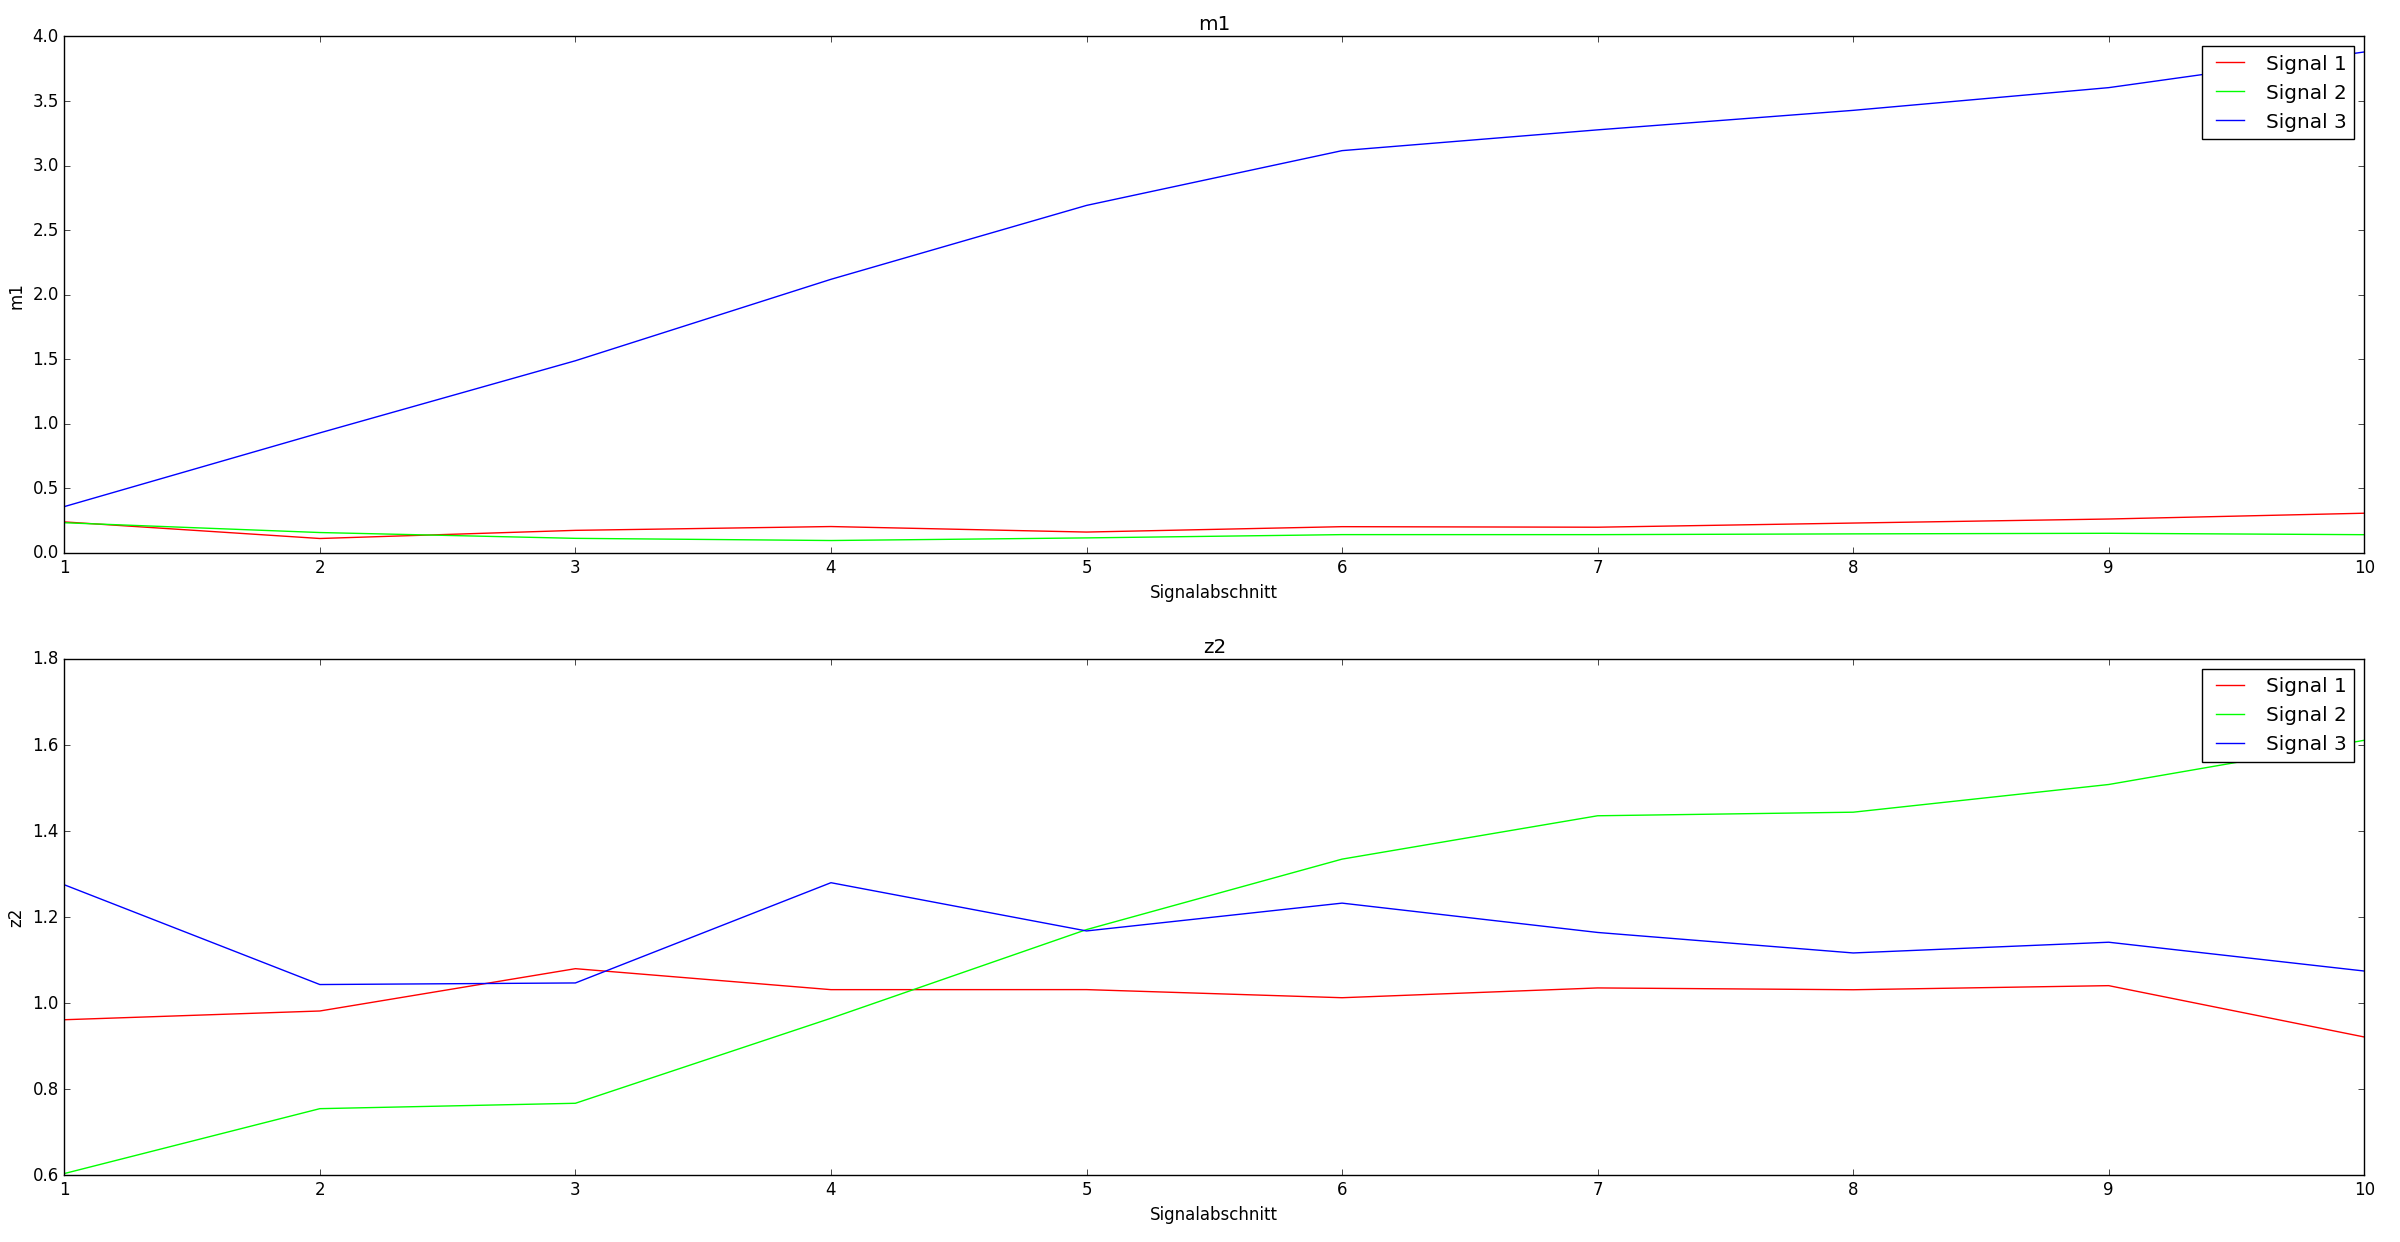
\includegraphics[width=1.0\textwidth]{A13.png}
        \caption{(13) $m_1$ und $z_2$ für Abschnitte von je 100 Messwerten}
        \label{fig:m1_z2_plt}
    \end{sidewaysfigure}
\end{document}
	\newpage
	\documentclass[fleqn,a4paper,12pt]{article}

%used Packages
\usepackage{standalone}		% Zum Einlesen aus anderen .tex-Files
\usepackage{geometry}		% Zur Bearbeitung des Layouts (Ränder,...)
\usepackage[german]{babel}
\usepackage[utf8]{inputenc}
\usepackage{amsmath}		% Mathematische Symbole
\usepackage{amssymb}     	% Nochmehr mathematische Symbole
\usepackage{dsfont}      	% Schriftsatz fuer Zahlenmengensymbole
%\usepackage{verbatim}   	% erweiterte Verbatim-Umgebung
\usepackage{alltt}       	% Quasi-Verbatim-Umgebung
\usepackage{fancyhdr}    	% Eigene Kopfzeilen
\usepackage{graphicx}    	% Zum Einbinden von Grafiken
							% Einbinden einer eps-Grafik geht so: includegraphics{path}
\usepackage{wrapfig}
\usepackage{lscape}
\usepackage{rotating}
\usepackage{epstopdf}

% Skalierung der Grafiken
\setlength{\unitlength}{1cm}

\frenchspacing               % Kein Extrafreiraum nach Satzzeichen
\setlength{\parindent}{0pt}  % Neue Absaetze nicht einruecken
%\sloppy                     % Schlampige Absatzformatierung
\fussy                       % Penible Absatzformatierung
\linespread{1.5}             % Zeilenabstand


% Seitenraender
\geometry{left=30mm, right=40mm, bottom=30mm}
				% Doc-class, Packageimports, fancy stuff
%%Seitenränder formatieren
\addtolength{\voffset}{-2cm}
\addtolength{\textheight}{0cm}
\addtolength{\hoffset}{0cm}
\addtolength{\textwidth}{2cm}
\addtolength{\headheight}{2cm} % fuer jeden Strichkode einen Zentimeter

% Font fuer Code 39
\font\xlix=wlc39 scaled 1200
\newcommand\barcode[1]{{\xlix@#1@}}

% Name, Matrikelnummer, Barcode
\newcommand\student[2]{
	\mbox{\scriptsize
		\begin{tabular}{@{}l@{}r@{}}
			\multicolumn{2}{@{}r@{}}{\barcode{#2}}\\
			#1&#2\\
		\end{tabular}}}

% Kopfzeile
\pagestyle{fancy}            % Eigene Kopfzeilen verwenden
\lhead{
	\small
	\textsc{Grundlagen der Signalverarbeitung \\
		WS 2017/2018 \\
		\"Ubung (\today)}
	\vfill}
\rhead{
	\begin{tabular}[b]{@{}rr@{}}
		\student{Philipp Badenhoop}{572693} &
		\student{Steven Lange}{568733} \\
		\student{Pascal Jochmann}{575056} &
		\student{Kevin Trogant}{572451}
\end{tabular}}			% Definition der Kopfzeile
%andere Definitionen
\providecommand{\R}{{\mathbb R}}
\providecommand{\N}{{\mathbb N}}
\providecommand{\Z}{{\mathbb Z}}
\providecommand{\Q}{{\mathbb Q}}
\providecommand{\C}{{\mathbb C}}
\providecommand{\F}{\mathcal{F}}
\providecommand{\less}{\setminus}
\providecommand{\inv}{{}^{-1}}
\providecommand{\Land}{\bigwedge}
\providecommand{\Lor}{\bigvee}			% Liste der zusätzlichen Commands und redefines

\begin{document}
    \section*{Übungsaufgabe 14}
    Die gegeben Messwerte (N=3):\\
    \begin{tabular}{|c| c| c|}
    	\hline
		\textbf{n}	&	\textbf{$t_n$}	&	\textbf{$f_n$}\\
		\hline
		0	&	-2	&	2\\
		1	&	0	&	1\\
		2	&	1	&	0
    \end{tabular}\\
	\begin{itemize}
		\item[a.]
		$f_{app}(t) = B_{M3} = \dots$\\
		$e_{B_{M3}}^2 = \dots$
		\item[b.]
		$f_{app}(t) = B_{M2} = \dots$\\
		$e_{B_{M2}}^2 = \dots$
		\item[c.]	
        \begin{align*}
            \begin{bmatrix}
                \Sigma_{n=0}^2 \Phi_{0,n} \Phi_{0,n}
            \end{bmatrix}
            \begin{bmatrix}
                c_0
            \end{bmatrix}
            &= \begin{bmatrix}
                \Sigma_{n=0}^2 f_n \Phi_{0,n}
            \end{bmatrix}
            \\
            \Longleftrightarrow \begin{bmatrix}
                3
            \end{bmatrix}
            \begin{bmatrix}
                c_0
            \end{bmatrix}
            &= \begin{bmatrix}
                3
            \end{bmatrix}
            \\
            \Longleftrightarrow 3c_0 &= 3 \Rightarrow c_0 = 1
        \end{align*}
        Also:
		$f_{app}(t) = B_{M1} = 1$\\
		$e_{B_{M1}}^2 = \dots$
		\item[d.] Das Interpolationspolynom nach Lagrange ist wie folgt definiert:
		\begin{align*}
			f_{app}(t) = L(t)	=& \sum_{i=0}^2 f_i\cdot \prod_{\substack{j=0\\i\ne j}}^2\frac{t - t_j}{t_i-t_j}\\
								=& 2\cdot\frac{t-0}{-2-0}\cdot\frac{t-1}{-2-1} + 1\cdot \frac{t+2}{0+2}\cdot\frac{t-1}{0-1} + 0\\
								=& 2\cdot\frac{-t}{2}\cdot\frac{1-t}{3} + \frac{t+2}{2}\cdot3\cdot\frac{1-t}{3}\\
								=& \frac{1-t}{3}\cdot\left(\frac{-2t+3t+6}{2}\right)\\
								=& \frac{t+6-t^2-6t}{6}\\
								=& \frac{-t^2-5t+6}{6}
		\end{align*}
	\end{itemize}
	\begin{figure}
%		\includegrapphic{A14_plot.png}
	\end{figure}
\end{document}

\end{document}